\section{prinsipiell løsning}
\label{sec:concept}


\subsection{Pseudotilfeldige signaler}
\label{sec:psedutolfeldigesig}

Fra oppgaven \cite{ntnu_2022_designprosjekt} blir det beskrevet at et deterministisk generert signal vil kunne gjenskapes dersom algoritmen brukt til å generere signalet er kjent, dermed så vil også signalet gjenta seg periodisk dersom det spilles av lenge nok. Disse signalene er ikke dermed ikke helt tilfeldige, men kan ta egenskaper som får dem til å virke tilfeldige. Dette kalles pseudotilfeldig og må oppfylle egenskapene:

\begin{enumerate}
    \item Perioden til signalet må være langt.
    \item Spekterert til signalet må være mest mulig flatt.
\end{enumerate}

kravene om lengde og flathet kommer an på applikasjonen der signalene skal brukes.

\subsection{Tilbakekoblet skiftregister}
\label{sec:tilbakekobling}

En kjent måte å generere pseudotilfeldige signaler på er ved bruk av tilbakekoblet skiftregiser som vist i figur \ref{fig:tilbakekoblet}. Her er det kaskadekoblet M + 1 skriftregistre av typen delay flip-flop. Her får $Q_M$ på inngangen et binært signal som funksjon av en eller flere av utgangene til utgangene til vippene $Q_{M-0}$ ved forrige klokkesignal.

\begin{figure}[!hbt]
	\centering
	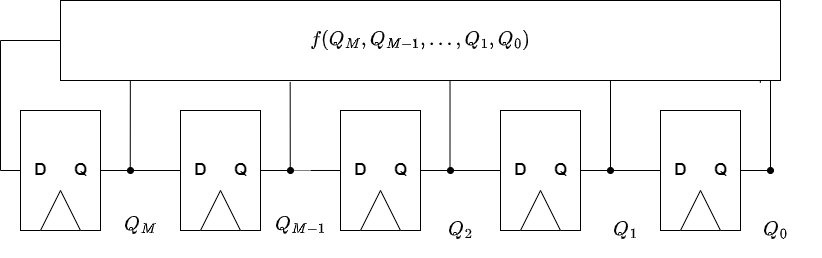
\includegraphics[scale=0.3]{./Images/02Concept/tilbakekoblet skiftregisker.drawio.png}
	\caption{Tilbakekoblet skiftregister av lengde M + 1.}
	\label{fig:tilbakekoblet}
\end{figure}

På vevsiden \cite{maxfield_2006_ee} blir det presentert et \textit{lineært tilbakekoblet skiftregister} (LFSR) der tilbakekoblingsfunksjonen er gitt ved en \textbf{XOR}-funksjon av et utvalg av utgangene. Ved å se på tabellen i siden blir det oppgitt av en LFSR på 32 Bits gir en sekvens med en maksimal lengde på 4294967295 dersom \textbf{XOR}-funksjonen tar inn utgangene fra vippe: 1, 5, 6, og 31 som vist i figur \ref{fig:LFSR}.

\begin{figure}[!hbt]
	\centering
	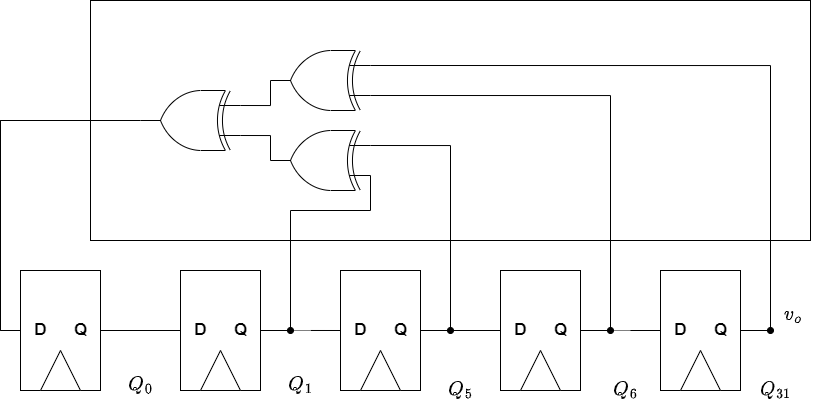
\includegraphics[scale=0.3]{./Images/02Concept/LFSR.png}
	\caption{Lineært tilbakekoblet skiftregister med 32 Bits.}
	\label{fig:LFSR}
\end{figure}

\subsection{MUX}
\label{sec:MUX}

Da skiftregistret inneholder bare nuller og \textbf{XOR}-funksjonen vil bare sende 0 dersom den kun tar inn 0. Dette kan løses ved å bruke en 2 til 1 multiplekser som er koblet til en bryter som vist i figur \ref{fig:MUX}


\begin{figure}[!hbt]
	\centering
	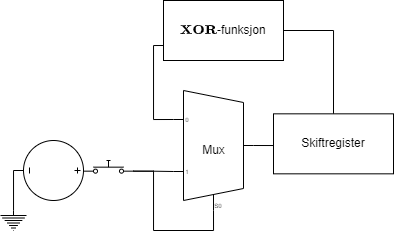
\includegraphics[scale=0.3]{./Images/02Concept/MUX.png}
	\caption{MUX med bryter for å få igang en sekvens.}
	\label{fig:MUX}
\end{figure}
